\begin{frame}
 \frametitle{Fundamental Symmetries in Physics: Parity $P$}
 \begin{block}{Electron scattering with accelerators (\textit{e.g.} Jefferson Lab)}
   Electrons strike a nucleus $N$ in a fixed target, not another electron beam, and we detect the scattered electrons
 \end{block}
 \begin{block}{Parity tests in electron scattering}
  \begin{itemize}
   \item \blue{Polarized electrons} (spin $\vec{S}$) on unpolarized target
   \item Instead of inverting $\vec{r} \rightarrow -\vec{r}$, $\vec{p} \rightarrow -\vec{p}$, and $\vec{S} \rightarrow \vec{S}$, \uncover<2>{we leave $\vec{r}$ and $\vec{p}$ unchanged but \alert{flip  polarization or spin $\vec{S}$}}
  \end{itemize}
 \end{block}
 \begin{center}
  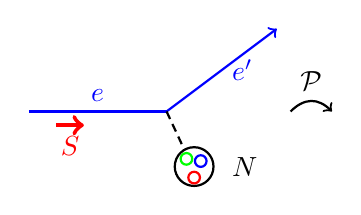
\begin{tikzpicture}[thick,scale=0.7]
   % Nucleon
   \draw (0,0) circle (10pt) node[right=10pt]{$N$};
   % Quarks
   \draw[red]   (0,-0.2) circle (3pt);
   \draw[green] (-0.14,0.14) circle (3pt);
   \draw[blue]  (0.12,0.10) circle (3pt);
   % Electron
   \draw[blue]      (-3,1) -- node[above]{$e$} (-0.5,1);
   \draw[blue,->] (-0.5,1) -- node[right]{$e'$} (1.5,2.5);
   % Electron spin
   \draw[ultra thick,red,->] (-2.5,0.75) -- node[below]{$S$} (-2,0.75);
   % Boson
   \draw[densely dashed] (-0.5,1) -- (-5pt,8.6pt);
   % Parity transformation
   \draw[->] (1.75,1.0) .. controls (2.0,1.25) and (2.25,1.25) .. node[above]{$\mathcal{P}$} (2.5,1.0);
  \end{tikzpicture}
  \only<1>{
  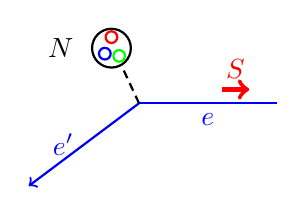
\begin{tikzpicture}[thick,scale=0.7]
   % Nucleon
   \draw (0,0) circle (10pt) node[left=10pt]{$N$};
   % Quarks
   \draw[red]   (0,0.2) circle (3pt);
   \draw[green] (0.14,-0.14) circle (3pt);
   \draw[blue]  (-0.12,-0.10) circle (3pt);
   % Electron
   \draw[blue]      (3,-1) -- node[below]{$e$} (0.5,-1);
   \draw[blue,->] (0.5,-1) -- node[left]{$e'$} (-1.5,-2.5);
   % Electron spin
   \draw[ultra thick,red,->] (2,-0.75) -- node[above]{$S$} (2.5,-0.75);
   % Boson
   \draw[densely dashed] (0.5,-1) -- (5pt,-8.6pt);
  \end{tikzpicture}
  }
  \only<2>{
  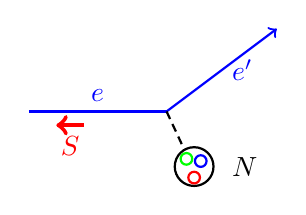
\begin{tikzpicture}[thick,scale=0.7]
   % Nucleon
   \draw (0,0) circle (10pt) node[right=10pt]{$N$};
   % Quarks
   \draw[red]   (0,-0.2) circle (3pt);
   \draw[green] (-0.14,0.14) circle (3pt);
   \draw[blue]  (0.12,0.10) circle (3pt);
   % Electron
   \draw[blue]      (-3,1) -- node[above]{$e$} (-0.5,1);
   \draw[blue,->] (-0.5,1) -- node[right]{$e'$} (1.5,2.5);
   % Electron spin
   \draw[ultra thick,red,->] (-2,0.75) -- node[below]{$S$} (-2.5,0.75);
   % Boson
   \draw[densely dashed] (-0.5,1) -- (-5pt,8.6pt);
  \end{tikzpicture}
  }
 \end{center}
\end{frame}
